%\subsection{Updated Byrd ice core chronology}\label{agedepthresults}
%\textbf{The 5,000-year accumulation function gives the best fit of the volcanic observations at the Byrd ice core, so it is used in the final ice flow model effort. The resulting uncertainties in radar depth and age to each of the layers of interest in shown in Table~\ref{tab:depthunc}. For the deepest observed reflector that can be traced between WAIS Divide ice core and Byrd ice core, the depth and age uncertainty are 0.3\% and 5\%, respectively, at the 1$\sigma$ level. The mean and median ages and depths are consistent due to the gaussian nature of the errors, as shown in Figure~\ref{fig:layer_agedepth}.}

Probability density functions generated by the metropolis algorithm sample uncertainty in the age and depth for each of four adar reflectors observed near the Byrd ice core. The results show the estimated age and depth converge to peaked gaussian distributions, with standard deviations generally increasing with depth and age as expected. The age of the observed reflectors increases dramatically with depth, with the oldest and deepest observed reflector dated to 35.43 $\pm$ 0.56 ka. These observed reflectors therefore span to before the Last Glacial Maximum.

%  %\begin{table}
%  \centering
%  \caption{ Depth and age mean, median, and uncertainty for ten strong radar reflectors near Byrd Station, West Antarctica. The radar two-way travel time (TWTT) is given in column 1. }
%  \begin{tabular}{ c c c c c c c}
%  \cline{1-7}
%  \multirow{2}{*}{Reflector} & TWTT& & Depth (m) & & Age  (a)& \\   
% % %& ($\mu$s)& Mean & Median & $\sigma$ & & Mean & Median & $\sigma$ \\
%  & ($\mu$s)& Mean  & $\sigma$ & &Mean  & $\sigma$ \\
%  \cline{3-4} \cline{6-7}
%   1 & 8.44    & 537.5  &  0.8 & &1200 & 20   \\
%   2 & 9.58    & 633.1  &  6.5 & &1770 & 40   \\
%   3 & 12.54   & 880.8  &  7.4 & &2100 & 60   \\
%   4 & 17.55   & 1300.7 &  6.1 & &3510 & 150  \\
%   5 & 22.42   & 1711.9 &  4.4 & &4360 & 200  \\
% %  %6 & 11.10  & 596.9  & 596.9  & 2.3 & &5440 & 5440 & 270   \\
% %  %7 & 12.78  & 738.8  & 738.8  & 2.3 & &7120 & 7110 & 370   \\
% %  %8 & 13.02  & 759.1  & 759.1  & 2.3 & 7350 & 7340 & 390   \\
% %  %9 & 18.92  & 1257.7 & 1257.7 & 2.4 & 16220 & 16300 & 1760   \\
% %  %10& 19.02  & 1266.2 & 1266.2 & 2.3 & 16400 & 16500 & 1820  \\
% % %\cline{1-7}
%  \end{tabular}
% % \tablenotetext{a}{Footnote text here.}
% % %\captionsetup{width=.9\textwidth}

%  %\label{tab:depthunc}
% %\end{table}




\begin{figure*}[h]
%\begin{center}
\centering
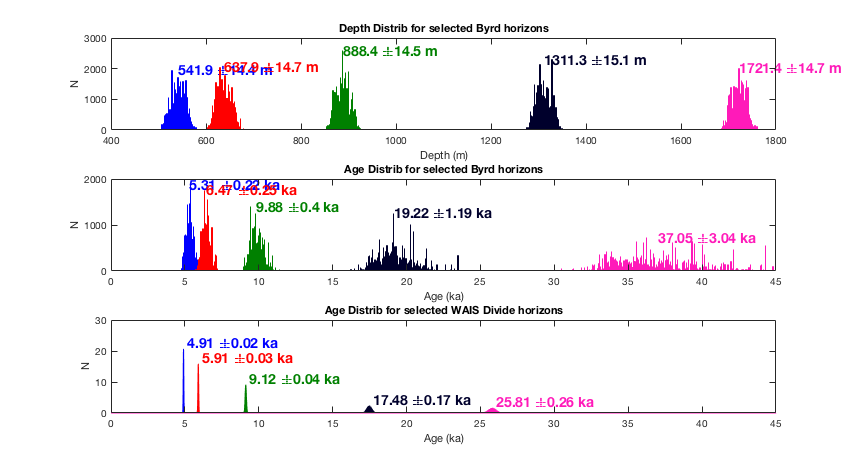
\includegraphics[scale=0.5]{figures/agedepthhisto}
%\captionsetup{width=.9\textwidth}
\caption[]{Age and depth distributions of 5 layers which can be traced between WAIS Divide and Byrd ice cores. The width of the histograms represents uncertainty in estimates of layer age and depth, which increase with depth as expected. }
%\end{center}
\label{fig:layer_agedepth}
\end{figure*}

\begin{figure*}[h]
%\begin{center}
\centering
\includegraphics[scale=0.3]{figures/spaghetti}
%\captionsetup{width=.9\textwidth}
\caption[]{Modeled age-depth relationship with uncertainty compared to measured volcanic chronology from \citet{hammer97}. }
%\end{center}
\label{fig:layer_agedepth}
\end{figure*}